

\begin{tabular}{c|c}
    $\lambda(x)$ & probability that item $x$ is harmful \\
    $h$ & per-item harm \\
    $P$ & demand  \\
    $F$ & fixed cost \\
    $\delta$ & externality \\
    $s$ & safe harbor threshold
\end{tabular}
% inspect/investigate/screen/filter

A platform hosts a continuum of user-generated content, with each item indexed by $x\in[0,1]$. 
Each item might cause harm $h$ with probability $\lambda(x)\in[0,1]$. Without loss of generality, we assume $\lambda(x)$ is a weakly increasing function such that the content is ordered by the ascending likelihood of causing harm. We also assume that there is no-harm content ($\lambda(0)=0$) and unambiguously harmful content ($\lambda(1)=1$).

% And items are heterogeneous in their probability of being harmful.

The inverse demand curve for the content is $Px$, interpreted as the marginal benefit from consuming the $x$-th unit of the content. We assume the demand curve is perfectly elastic such that the marginal consumer benefit is constant at $P$.
There is a fixed cost $F$ of starting up the platform, regardless of how many items of content it hosts.

Content removal decision is modeled as a threshold $\hat{x}\in[0,1]$ such that items $x>\hat{x}$ are removed and items $x\ls\hat{x}$ remains on the platform. 
\footnote{Choosing a threshold is without loss of generality. One can show that removing any subset of the content $\mathcal{X}\subset[0,1]$ is a weakly dominated strategy.}
Given $\hat{x}$, $\int_0^{\hat{x}}\lambda(x)hdx$ is the expected harm given the amount of content $\hat{x}$, and $P\hat{x}$ is the consumer welfare.
The social welfare function is given by 
\begin{equation}\label{eqn:efficiency_1}
    \max\{\max_{\hat{x}}P\hat{x} - \int_0^{\hat{x}}h\lambda(x)dx-F, 0\}.
\end{equation}
Suppose the platform does not shut down, 
the efficient moderation decision $x^e$ is such that
\begin{equation}
    \lambda(x^e)=\frac{P}{h},
\end{equation}
where $P$ is the marginal cost of removing the marginal item $x^e$, and $\lambda(x^e)h$ is the marginal social benefit of removing $x^e$. 
If the triple $(h,P,F)$ is such that $Px^e - \int_0^{x^e}h\lambda(x)dx < F$, social efficiency requires the platform to shut down and carry no content. If instead the triple $(h,P,F)$ is such that $Px^e - \int_0^{x^e}h\lambda(x)dx \gs F$, social efficiency requires the platform to operate but only carries content $[0,x^e]$.

Intermediary immunity $d=0$.
The platform is profit-maximizing. Since the prevailing market price is $P$, the revenue is $P\hat{x}$, the profit function is given by 
\begin{equation}
    \max\{\max_{\hat{x}}P\hat{x}-F,0\}.
\end{equation}
Suppose $P<F$, the platform shuts down. Suppose $P\gs F$, the profit-maximizing choice is $x^{\ast}=1$ such that the platform keeps all of the content. Without the threat of liability, the platform has no incentive to remove any of the harmful content. 


A regulator would like to maximize social welfare from the content carried on the platform. It cannot directly control which items are carried and which are removed. Instead, it can impose a liability $d\ge 0$ on the platform for each item of harmful content the platform carries. The regulator's optimization problem is to choose a value of $d$ that will induce the platform to maximize the social welfare.

Under strict liability, the platform always pays damages $d$ due to the harm caused by the content it hosts. 
The platform's profit maximization problem then becomes
\begin{equation}\label{eqn:platform_1}
    \max\{\max_{\hat{x}}P\hat{x} - \int_0^{\hat{x}}d\lambda(x)dx-F, 0\}.
\end{equation}
Comparing the objective function \ref{eqn:efficiency_1} and the profit function \ref{eqn:platform_1}, we have that the platform's moderation decision $x^{\ast}$ is efficient if $d=h$. 
That is, the optimal level of damages paid by the platform is equal to the harm.
If so, strict liability rule on the platform leads to social optimum. 

\begin{proposition}
Strict liability leads to the efficient moderation outcome.
\end{proposition}

Other parameters may determine whether it is socially efficient to remove none, part, or all of the content. But no matter what that efficient outcome is, strict liability (d=h) will perfectly align the incentive of the platform with that of a social planner.

Safe harbor provision combines both features of strict liability and immunity. 
\begin{equation}
d=
\lt\{\begin{array}{ll}
    h & \mbox{if $\int_0^{\hat{x}}\lambda(x)hdx>s$}, \\
    0 & \mbox{otherwise}.
\end{array}\rt.
\end{equation}
If the total harm on the platform exceeds the threshold $s$, the platform loses its safe harbor status and will be held strictly liable for the content. Otherwise, the platform will be immune from any liability. 

Must remove rule
\begin{equation}
d=
\lt\{\begin{array}{ll}
    h & \mbox{if $\hat{x}>x^e$}, \\
    0 & \mbox{otherwise}.
\end{array}\rt.
\end{equation}
Safe harbor provision also leads to social optimum. Q. loss of safe harbor means all the content is liable for $d$, or only part of the content liable for $d$.

Positive externality . The postive externality could be the knowledge spillover, the democratic value of the institution, etc.

\begin{proposition}
If $\delta\gs h-P$, intermediary immunity leads to the efficient moderation outcome.    
\end{proposition}


Platform 




HERE






\begin{figure}[h]
    \centering
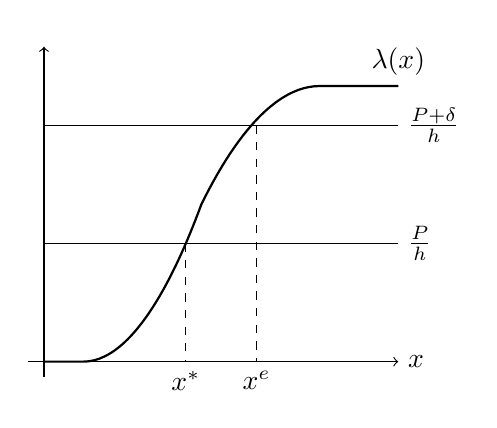
\begin{tikzpicture}[scale=1]
    \draw[->] (-0.2,0) -- (4.5,0) node[right]{$x$}; 
    \draw[->] (0,-0.2) -- (0,4) node[above]{};
    \draw[thick] (0,0) to (0.5,0) parabola (2,2) parabola[bend at end] (3.5,3.5) to (4.5,3.5) node[above]{$\lambda(x)$};
    \draw[thin] (0,1.5) to (4.5,1.5) node[right]{$\frac{P}{h}$};
    \draw[dashed, thin] (1.8,1.5) -- (1.8,0) node[below]{$x^*$}; 
    \draw[thin] (0,3) to (4.5,3) node[right]{$\frac{P+\delta}{h}$};
    \draw[dashed, thin] (2.7,3) -- (2.7,0) node[below]{$x^e$}; 
\end{tikzpicture}
    \caption{Platform Over-Removal under Strict Liability if $\delta>0$}
    \label{fig:removal}
\end{figure}



\begin{figure}[h]
    \centering
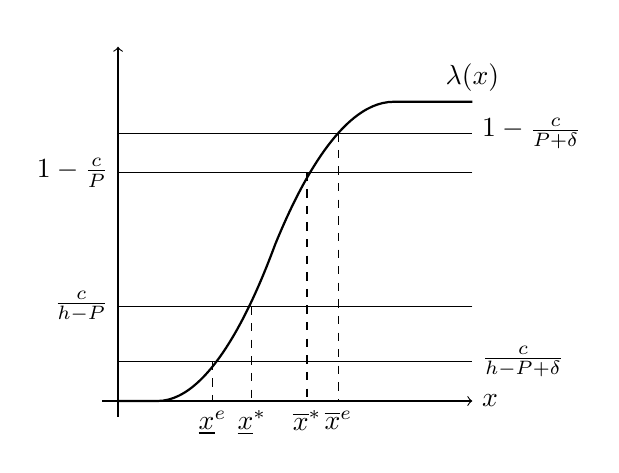
\begin{tikzpicture}[scale=1]
    \draw[->] (-0.2,0) -- (4.5,0) node[right]{$x$}; 
    \draw[->] (0,-0.2) -- (0,4.5) node[above]{};
    \draw[thick] (0,0) to (0.5,0) parabola (2,2) parabola[bend at end] (3.5,3.8) to (4.5,3.8) node[above]{$\lambda(x)$};
    %% next four \draw are efficiency
    \draw[thin] (0,0.5) to (4.5,0.5) node[right]{$\frac{c}{h-P+\delta}$};  
    \draw[thin] (0,3.4) to (4.5,3.4) node[right]{$1-\frac{c}{P+\delta}$};
    \draw[dashed, thin] (1.2,0.5) -- (1.2,0) node[below]{$\underline{x}^e$};
    \draw[dashed, thin] (2.8,3.4) -- (2.8,0) node[below]{$\overline{x}^e$};
    %% next four \draw are profit
    \draw[thin] (4.5,1.2) to (0,1.2) node[left]{$\frac{c}{h-P}$};  
    \draw[thin] (4.5,2.9) to (0,2.9) node[left]{$1-\frac{c}{P}$};
    \draw[dashed, thin] (1.7,1.2) -- (1.7,0) node[below]{$\underline{x}^{\ast}$};
    \draw[dashed, thin] (2.4,2.9) -- (2.4,0) node[below]{$\overline{x}^{\ast}$};   
\end{tikzpicture}
    \caption{Platform Under-investigate under Strict Liability if $\delta>0$}
    \label{fig:investigation}
\end{figure}












%% The platform receives a revenue of $R \ge 0$ for each item it carries, good or bad. It can tell the difference between the two types at a cost of $C \ge 0$ per item. If it decides to remove an item of content, it gives up the revenue associated with that item.






\iffalse


The platform has three viable strategies:
\begin{itemize}

\item  \emph{First}, the platform can carry all content, good and bad, and make no attempt to tell the two apart. If it does so, it receives $nR$ in revenue (for all the content) but pays $n\beta L$ in liability (for the bad content) for a net profit of
\begin{equation}
\label{profitnofilter}
nR - n\beta L
\end{equation}
If the platform carries all content, society realizes a total benefit of $n(1-\beta)G$ from the good items, but a harm of $n\beta B$ from the bad items. Overall social welfare is thus
\begin{equation}
\label{welfarenofilter}
n(1-\beta)G - n \beta B
\end{equation}

Suppose the platform can pay an inspection cost $c$ per item to observe a signal of item $x$ indicating whether $x$ is harmful or not. In this case, if the platform chooses to investigate, it can condition its removal decision upon the realization of the signal. 

The signal is useful only if the 
For $x\ls \hat{x}$, the signal is useful if it reveals the item $x$ is harmful and thus should be removed instead. In this case, investigation prevents the welfare loss of under-removal. 



\item \emph{Second}, the platform can pay $nC$ to inspect every item of content to discover whether it is good or bad. Once it has done so, it carries the good items for a total of $n(1-\beta)R$ in revenue, but removes the bad items (forgoing $n\beta R$ in revenue). Its net profit is therefore 
\begin{equation}
\label{profitfilter}
n(1 - \beta)R - nC    
\end{equation}
If the platform filters, society still realizes the benefit of  $n(1-\beta)G$ from the good items of content, but no harm because the bad items have been removed. Social welfare is
\begin{equation}
\label{welfarefilter}
n(1-\beta)G
\end{equation}

%% platform pay cost c to observe a signal

\end{itemize}

\section{The Regulator's Goals}

Filtering (equation~\ref{welfarefilter}) is always the regulator's preferred outcome. It is better than no filtering (equation~\ref{welfarenofilter}) as long as there is any bad content ($\beta > 0$) and that content causes harm ($B > 0$). It is better than shutdown (equation~\ref{welfareshutdown}) as long as there is any good content ($\beta < 1$) and that content creates benefits ($G > 0$).

The regulator's second choice, however, depends on the prevalence $\beta$ of bad content. Social welfare is higher with no filtering than with shutdown as long as $n(1-\beta)G - n \beta B > 0$. In words, an unfiltered platform does more good than harm as long as there is enough good content as compared with bad to outweigh the cost of bad content as compared with good. Rearranging and solving for $\beta$, this indicates that the regulator should prefer to have the platform operate as long as
\begin{equation}
\label{welfarefvs}
\beta \;<\; \frac{G}{B+G}
\end{equation}
When $B=G$, i.e. the cost of an item of bad content exactly equals the benefit of an item of good content, equation~\ref{welfarefvs} indicates that $\beta < \frac{1}{2}$, i.e. there must be less bad content then good. When $B \gg G$, i.e., each item of bad content causes much more harm than each item of good content creates benefit, $\beta$ approaches $0$, i.e., there must be much less bad content than good. When $B \ll G$, i.e. each item of bad content causes much less harm than each item of good content creates benefit, $\beta$ approaches $1$, i.e., there can be much more bad content than good.

\section{The Platform's Incentives}

Now consider things from the platform's perspective.  Its choices depend on the value of $L$. The platform will prefer to filter (rather than leaving all content up) if its profit with filtering (equation \ref{profitfilter}) exceeds its profit without filtering but with liability (equation \ref{profitnofilter}), i.e. if $nR(1 - \beta) - nC >  nR - nL\beta$. Rearranging and solving for $L$,  this condition is equivalent to 
\begin{equation}
\label{dofilter}
L \;>\; R + C\frac{1}{\beta}
\end{equation}
That is, the liability $L$ for each item of bad content must not only exceed the platform's revenue $R$ for that item, but also the cost of filtering. That cost is not just $C$, the cost to inspect one item, since the platform must inspect \emph{every} item in order to find the bad ones. This filtering cost per bad item increases as the proportion of bad items decreases. If one half of all items are bad, then the  liability must be greater than $R + 2C$. If one millionth of all items are bad, the liability must be greater than $R + 1,000,000C$. Thus, when the prevalence of bad content is sufficiently low, a rational platform  will prefer to take the occasional liability hit rather than spend exorbitant sums searching for needles in haystacks.  

Since the regulator always prefers filtering to no filtering, it might seem that it should simply set $L$ high enough to induce filtering. Unfortunately, this strategy can backfire, since the platform has a third option open: shutting down. It will operate with filtering only as long as its expected profits with filtering are positive, i.e. when $n(1 - \beta)R - nC > 0$. Solving for $C$ gives 
\begin{equation}
\label{doshutdown}
C \;<\; (1 - \beta) R
\end{equation}
I.e., operating with filtering is uneconomical if the revenue from the good items is insufficient to pay for filtering all of the items. For any given $\beta$ and $R$, there is some critical upper limit of $C$ at which the platform cannot break even with filtering. Call this limit $C^*$; it is equal to $(1-\beta) R$. If $L$ has been set so high that the platform is better of filtering than not filtering, the platform is also better off shutting down than not filtering.

That is, if the per-item cost of filtering $C$ is above the critical value $C^*$ there is no value of $L$ through which the regulator can induce the platform to filter. The platform is always better off either leaving all the content up or taking all of it down. The cost of sifting through it to distinguish the good content from the bad is simply too high.

Society would prefer that the platform filter rather than leaving all content up, and it can raise the liability $L$ high enough to make the platform prefer to filter, too. But if the platform also prefers to shut down rather than filter, because filtering would push its profits below zero, that level of liability will induce the platform to shut down. The threat of liability only works to induce filtering if it leaves the platform with a profitable option. 

In this situation where $C > C^*$, the regulator still has a choice to make. It can set $L$ high enough to actually force the platform to shut down, or it can set $L$ low enough to allow the platform to operate and accept that it will not filter out the bad items of content. It should choose based on equation~\ref{welfarefvs}, i.e. based on whether the platform overall is beneficial or harmful.

Putting this all together, the case for intermediary immunity is justified when $C > C^*$ and $\beta < G/(B+G)$ Effective filtering is cost-prohibitive, so that imposing liability will lead the platform to overfilter (from society's point of view) by shutting down. But since society prefers to have the platform to not having it (because the good content still outweighs the bad), it is better off with underfiltering than overfiltering.


\fi



(i) If all the platform can do is content removal and no positive externality, strict liability leads to efficiency.
(ii) content removal + positive externality, strict liability leads to over-removal and immunity might be justified if the externality is sufficiently large (though that means keeping all the content).
(iii) If platform can first choose whether to investigate and then decide on removal, with no positive externality, strict liability again leads to efficiency !
(iv) investigate + removal + positive externality, strict liability leads to under-investigation and over-removal.  
(v) imperfect signal does not change (iii) and (iv). 




Filtering costs $L_0 + nL$ where $n$ is the number of items filtered.



% explain independent of h




Different levels of liability (e.g. loss of safe harbor, conditional immunity)


effort as investigation 
notice upon takedown

must carry or must remove rule

Next steps:
(1) Social planner chooses safe harbor level
(2) Platform has fixed costs to operate
(3) Platform can invest to create a better filter